\documentclass{standalone}
\usepackage{tikz, ifthen}
\usepackage{amsmath}
\usetikzlibrary{decorations.pathreplacing}

\begin{document}

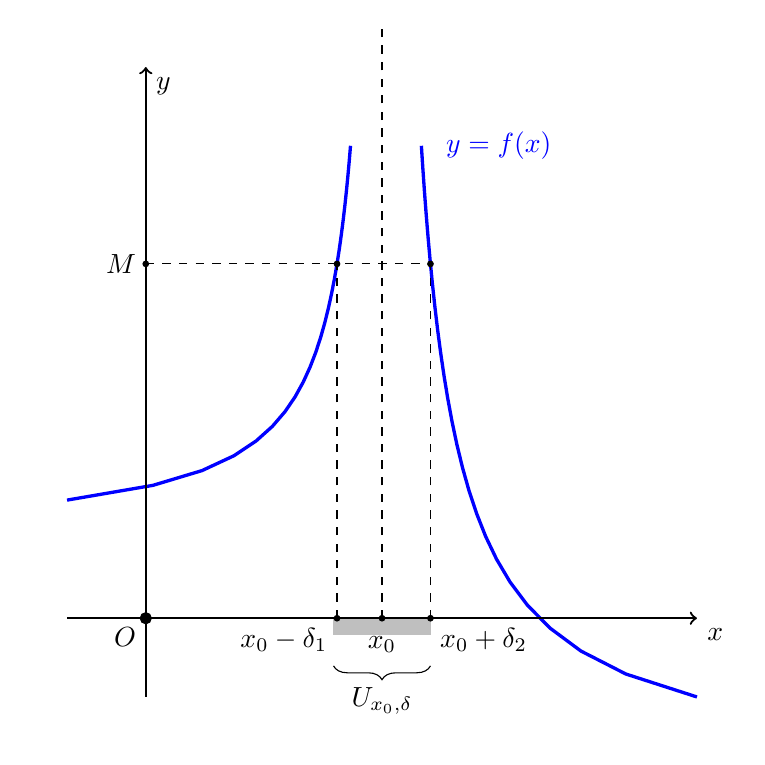
\begin{tikzpicture}
    
    % Center of the circle
    \def\xmin{-1}
    \def\xmax{7}
    \def\ymin{-1}
    \def\ymax{7}
    \def\dx{.5}
    \def\dy{.5}
    \def\xminb{\xmin-\dx}
    \def\xmaxb{\xmax+\dx}
    \def\yminb{\ymin-\dy}
    \def\ymaxb{\ymax+\dy}
    \def\xo{2}     % translation, x
    \def\yo{1.5}   % translation, y
    \def\xpmin{-6}
    \def\xpmax{ 6}
    \def\ypmin{-5.5}
    \def\ypmax{ 5.5}
    \def\epsil{.2}   % espil = .8 .5 .2
    \def\yo{4.5}
    % \def\delta{1}

    % Fill outside region
    \clip (\xminb, \yminb) rectangle (\xmaxb, \ymaxb);
    \draw[white, fill=white] (\xminb, \yminb) rectangle (\xmaxb, \ymaxb);

%   % Draw grid
%   \draw[step=1., gray!60, ultra thin] (\ymi22n-1, \xmin-1) grid (\ymax+1, \ymax+1); % Visible grid with lighter color
    
    % Graph
    \draw[very thick, blue] plot[parametric, domain=1.5:6] ({(-2/(\x-1)+3)}, {\x}); % Branch 1
    \draw[very thick, blue] plot[parametric, domain=-1:6] ({(4./(\x+2)+3)}, {\x}) node[right=5pt] {$y=f(x)$}; % Branch 1
    \coordinate (B)  at ({3},0);
    \coordinate (A)  at ({3}, {\ymax+3});
    \coordinate (C)  at (0,{\yo});    
    \coordinate (A1) at ({(-2/(\yo-1)+3)},{\yo}); 
    \coordinate (A2) at ({(4./(\yo+2)+3)}, {\yo}); 
    \coordinate (B1) at ({(-2/(\yo-1)+3)}, 0); 
    \coordinate (B2) at ({(4./(\yo+2)+3)}, 0); 
    \coordinate (D1) at ({2*(3)-(4./(\yo+2)+3)},0);    
    \coordinate (B2s) at ({(4./(\yo+2)+3)}, -0.2); 
    \coordinate (D1s) at ({2*(3)-(4./(\yo+2)+3)}, -0.2);    
%   coordinate (D1s) at ({2*(.2*\yo*\yo-0.5)-(.2*\yb*\yb-0.5)},-.2);    
%   \coordinate (B2s) at ({(.2*\yb*\yb-0.5)},-.2);    
%   \coordinate (A1) at ({.2*\ya*\ya-0.5},{\ya}); 

    % U(x0,delta)
    \draw[gray!50, fill=gray!50] (D1) -- (B2) -- (B2s) -- (D1s) -- cycle ;

    % Axes, x
    \draw[->, thick, black] (\xmin, 0) -- (\xmax, 0) node[below right] {$x$};
    \draw[->, thick, black] (0, \ymin) -- (0, \ymax) node[below right] {$y$};

%   \draw[dashed] (C)  -- (A1) ;
    \draw[dashed] (C)  -- (A2) ;
    \draw[dashed] (B)  -- (A);
    \draw[dashed] (B1) -- (A1); 
    \draw[dashed] (B2) -- (A2); 
%   \draw[dashed] (C1) -- (A1);
%   \draw[dashed] (C2) -- (A2);

    \filldraw[black] (A) circle (1pt);
    \filldraw[black] (B) circle (1pt) node[below = 3pt] {$x_0$};
    \filldraw[black] (C) circle (1pt) node[left] {$M$};
    \filldraw[black] (A1) circle (1pt);
    \filldraw[black] (A2) circle (1pt);
    \filldraw[black] (B1) circle (1pt) node[below left ] {$x_0-\delta_1$};
    \filldraw[black] (B2) circle (1pt) node[below right] {$x_0+\delta_2$};
%   \filldraw[black] (C1) circle (1pt) node[below left] {$L-\varepsilon$};
%   \filldraw[black] (C2) circle (1pt) node[above left] {$L+\varepsilon$};

    \draw [decorate,decoration={brace,amplitude=5pt,mirror,raise=4ex}]
      (D1) -- (B2) node[midway,yshift=-30pt]{$U_{x_0,\delta}$};

%   % Axis ticks
%   \foreach \x in {\xmin,..., \xmax}{
%       \ifthenelse{ \x = 0 }{}{\draw[black] (\x, -0.1) -- (\x, +0.1) node[below=8pt, left=0pt] {\small $\x$};}
%  }
%   \foreach \y in {\ymin,..., \ymax}{
%       \ifthenelse{ \y = 0 }{}{\draw[black] (-0.1, \y) -- (0.1, \y) node[left=4pt] {\small $\y$};}
%   }
    
    % Origin
    \filldraw[black] (0,0) circle (2pt) node[below left] {$O$};

%   \filldraw[blue]  (3,5) circle (1pt) node[below right] {$\equiv (3,5)$};
%   \filldraw[black] (3,5) circle (2pt) node[below right] {$A \equiv (3,5)$};

%   \filldraw[blue]  (-4,3) circle (1pt) node[below right] {$\equiv (-4,3)$};
%   \filldraw[black] (-4,3) circle (2pt) node[below right] {$B \equiv (-4,3)$};

%   \filldraw[blue]   (1,-4) circle (0pt) node[above right=8pt] {$\qquad \ 1$};
%   \filldraw[purple] (1,-4) circle (0pt) node[above right=8pt] {$\qquad \quad \ -4$};
%   \filldraw[black]  (1,-4) circle (2pt) node[above right] {$C \equiv (1,-4)$};

%   % Foci
%   \filldraw[blue] (\xa, \ya) circle (2pt) node[above right] {$0$};
%   \filldraw[blue] (\xb, \yb) circle (2pt) node[above right] {$2$};
    
\end{tikzpicture}

\end{document}
